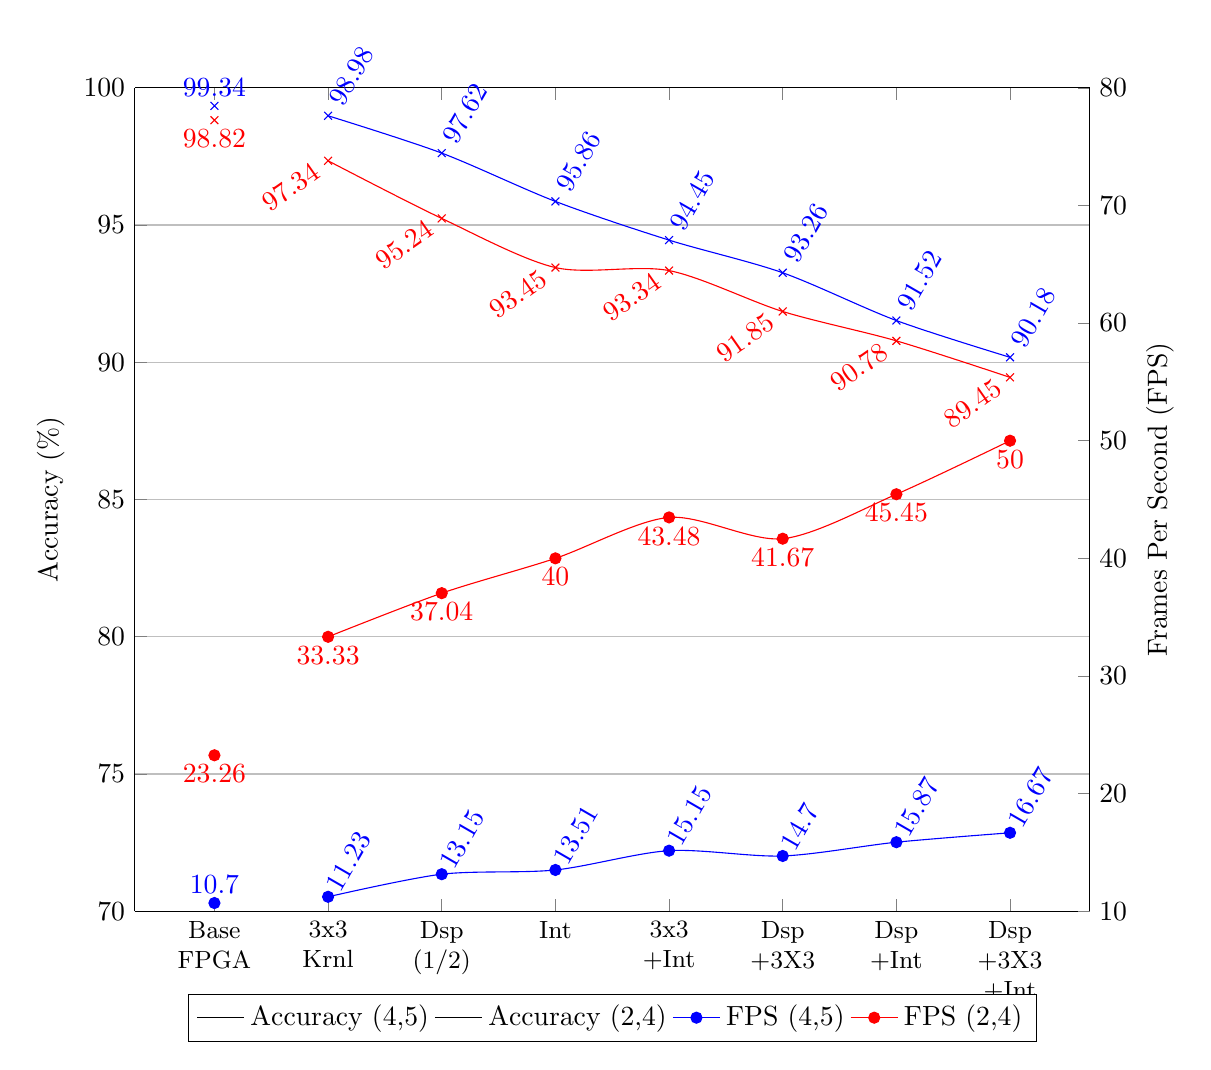
\begin{tikzpicture}
\pgfplotsset{
    scale only axis,
    scaled x ticks=base 10:3,
}
\begin{axis}[
  width=\textwidth, % Adjust the width here
  axis y line*=left,
  ymin=70, ymax=100,
  ymajorgrids = true,
  legend style={at={(0.5,-0.10)},
      anchor=north,legend columns=-1},%
  symbolic x coords={Base\\FPGA,3x3\\Krnl, Dsp\\ (1/2),Int,3x3\\  +Int, Dsp\\ +3X3,Dsp\\ +Int,Dsp\\ +3X3\\ +Int},
    xtick distance=1,
    nodes near coords,
    x tick label style={font=\small,align=center},
  ylabel=Accuracy (\%),
]

%\node[label=(Base 2,4),fill,inner sep=2pt,mark=x,red] at (axis cs:0,99.34) {};
%\node[label=(Base 3,4),fill,inner sep=2pt,mark=x,blue] at (axis cs:0,98.82) {};

\addplot[nodes near coords style={anchor=west,rotate=60,inner xsep=5pt},smooth,mark=x,blue]
  coordinates{
    (3x3\\Krnl,98.98)
    (Dsp\\ (1/2),97.62)
    (Int,95.86)
    (3x3\\  +Int,94.45)
    (Dsp\\ +3X3,93.26)
    (Dsp\\ +Int,91.52)
    (Dsp\\ +3X3\\ +Int,90.18)

}; \label{plot_one}


\addplot[nodes near coords style={anchor=south,rotate=0,inner xsep=5pt},smooth,mark=x,blue]
  coordinates{
(Base\\FPGA,99.34)
}; 

\addplot[nodes near coords style={anchor=north,rotate=0,inner xsep=10pt},smooth,mark=x,red]
  coordinates{
(Base\\FPGA,98.82)
}; 


\addplot[nodes near coords style={anchor=east,rotate=35,inner xsep=5pt},smooth,mark=x,red]
  coordinates{
    (3x3\\Krnl,97.34)
    (Dsp\\ (1/2),95.24)
    (Int,93.45)
    (3x3\\  +Int,93.34)
    (Dsp\\ +3X3,91.85)
    (Dsp\\ +Int,90.78)
    (Dsp\\ +3X3\\ +Int,89.45)
}; \label{plot_two}

\end{axis}

\begin{axis}[
  width=\textwidth, % Adjust the width here
  axis y line*=right,
  axis x line=none,
  legend style={at={(0.5,-0.10)},
      anchor=north,legend columns=-1},
  symbolic x coords={Base\\FPGA, 3x3\\Krnl, Dsp\\ (1/2),Int,3x3\\  +Int, Dsp\\ +3X3,Dsp\\ +Int,Dsp\\ +3X3\\ +Int},
 xtick=data,
  nodes near coords,
  ymin=10, ymax=80,
  ylabel=Frames Per Second (FPS)
]
\addlegendimage{/pgfplots/refstyle=plot_one}\addlegendentry{Accuracy (4,5)}
\addlegendimage{/pgfplots/refstyle=plot_two}\addlegendentry{Accuracy (2,4)}

\addplot [nodes near coords style={anchor=west,rotate=60,inner xsep=3pt},smooth,mark=*,blue]
  coordinates{
    (3x3\\Krnl,11.23)
    (Dsp\\ (1/2),13.15)
    (Int,13.51)
    (3x3\\  +Int,15.15)
    (Dsp\\ +3X3,14.70)
    (Dsp\\ +Int,15.87)
    (Dsp\\ +3X3\\ +Int,16.67)
};\addlegendentry{FPS (4,5)}

\addplot[nodes near coords style={anchor=north,rotate=0,inner xsep=3pt},smooth,mark=*,red]
  coordinates{
    (3x3\\Krnl,33.33)
    (Dsp\\ (1/2),37.04)
    (Int,40)
    (3x3\\  +Int,43.48)
    (Dsp\\ +3X3,41.67)
    (Dsp\\ +Int,45.45)
    (Dsp\\ +3X3\\ +Int,50)
}; \addlegendentry{FPS (2,4)}




\addplot[nodes near coords style={anchor=south,rotate=0,inner xsep=5pt},smooth,mark=*,blue]
  coordinates{
(Base\\FPGA,10.7)
}; 

\addplot[nodes near coords style={anchor=north,rotate=0,inner xsep=5pt},smooth,mark=*,red]
  coordinates{
(Base\\FPGA,23.26)
}; 


\end{axis}

\end{tikzpicture}